%%%%%%%%%%%%%%%%%%%%%%%%%%%%%%%%%%%%%%%%%
%  My documentation report
%  Objetive: Explain what I did and how, so someone can continue with the investigation
%
% Important note:
% Chapter heading images should have a 2:1 width:height ratio,
% e.g. 920px width and 460px height.
%
%%%%%%%%%%%%%%%%%%%%%%%%%%%%%%%%%%%%%%%%%

%----------------------------------------------------------------------------------------
%	PACKAGES AND OTHER DOCUMENT CONFIGURATIONS
%----------------------------------------------------------------------------------------

\documentclass[11pt,fleqn]{book} % Default font size and left-justified equations

\usepackage[top=3cm,bottom=3cm,left=3.2cm,right=3.2cm,headsep=10pt,letterpaper]{geometry} % Page margins
\usepackage[dvipsnames]{xcolor}
\usepackage{lipsum} % Required for specifying colors by name

% Font Settings
\usepackage{avant} % Use the Avantgarde font for headings
%\usepackage{times} % Use the Times font for headings
\usepackage{mathptmx} % Use the Adobe Times Roman as the default text font together with math symbols from the Symbol, Chancery and Computer Modern fonts

\usepackage{microtype} % Slightly tweak font spacing for aesthetics
\usepackage[utf8]{inputenc} % Required for including letters with accents
\usepackage[T1]{fontenc} % Use 8-bit encoding that has 256 glyphs

\usepackage[french]{varioref}
\usepackage[french]{babel}

\usepackage{wrapfig}
\usepackage{listings}
\usepackage{multicol}
\usepackage{multirow}
\usepackage{colortbl}
\usepackage{booktabs}
\newcommand{\tabitem}{~~\llap{\textbullet}~~}
\usepackage{hyperref}
\usepackage{qrcode}
\usepackage{soul}
\usepackage{tabto}
\usepackage{multienum}


\definecolor{deepblue}{rgb}{0.0,0.0,0.5}
\definecolor{deepred}{rgb}{0.6,0,0}
\definecolor{deepgreen}{rgb}{0,0.5,0}
\definecolor{ocre}{RGB}{51,102,0} 
\definecolor{lightgray}{RGB}{229,229,229} 
\definecolor{palerod}{RGB}{238,232,170}
\definecolor{verttelecom}{RGB}{171,180,0}

\newcommand\pythonstyle{\lstset{
language=Python,
basicstyle=\ttfamily\footnotesize,
morekeywords={self},              % Add keywords here
frame=tb,                         % Any extra options here
showstringspaces=false
}}

\definecolor{backcolour}{rgb}{0.95,0.95,0.92}

\newcommand\termctyle{\lstset{
frame=tb,                         % Any extra options here
showstringspaces=false
}}


% Python environment
\lstnewenvironment{python}[1][]
{
\pythonstyle
\lstset{#1}
}
{}

\lstnewenvironment{termc}[1][]
{
\lstset{#1}
}
{}


% RFC
\newcommand\rfc[1]{\href{http://www.ietf.org/rfc/rfc#1.txt}{\textcolor{blue}{RFC #1}\index{RFC #1}}}
\newcommand\pfunction[2]{\texttt{#2}\index{Module Python!#1!#2}}

% boot.py

\newcommand\glos[1]{\gls{#1}\index{#1}}
\newcommand\pprog[2]{\href{https://github.com/ltn22/PLIDObis/blob/master/#2/#1}{\texttt{#1}}\index{Programmes Python!#1}}
\newcommand\lprog[2]{\href{https://github.com/ltn22/PLIDObis/blob/master/#2/#1}{\texttt{#1}}\index{Programmes micro-python!#1}}

% QUESTION

\usepackage[most]{tcolorbox}
\usepackage{ifthen}

\provideboolean{Response}\setboolean{Response}{true}

\newcommand{\Correct}[1]{\ifthenelse{\boolean{Response}}{#1}{\textbf{#1}}}
\newcommand{\Wrong}[1]{\ifthenelse{\boolean{Response}}{#1}{\textcolor{black!20}{#1}}}

\newwrite\tempfile
\immediate\openout\tempfile=questions.tex


\newtcbtheorem[auto counter,number within=section]{theo}%
  {Question}{fonttitle=\bfseries\upshape, 
     arc=0mm, colback=blue!5!white,colframe=blue!75!black}{Question}
     
\newcommand\Question[3]{
\begin{theo}{#1}{summation}
#2
\immediate\write\tempfile{\noexpand\textbf{Question \thetcbcounter {} page \thepage} {} }
\immediate\write\tempfile{\unexpanded{#2}\noexpand\vspace{1em}\noexpand\newline}
\immediate\write\tempfile{\unexpanded{#3}\noexpand\newline\noexpand\newline}

\end{theo}
}

% MATHS PACKAGE
\usepackage{amsmath,tikz}
\usetikzlibrary{matrix}
\newcommand*{\horzbar}{\rule[0.05ex]{2.5ex}{0.5pt}}
\usepackage{calc}

% VERBATIM PACKAGE
\usepackage{verbatim}

\usepackage{tikz}

\usetikzlibrary{automata}
\usetikzlibrary[shadows]
\usetikzlibrary{shapes}
\usetikzlibrary[decorations.footprints] 
\usetikzlibrary{decorations.pathmorphing}
\usetikzlibrary{decorations.pathreplacing}
\usetikzlibrary{decorations.text}
\usetikzlibrary {arrows}
\usetikzlibrary{patterns}
\usetikzlibrary{calc}
\usetikzlibrary{external}

\usepackage{tikz-timing}

% Acronyms

\usepackage{makeidx}
\makeindex

\usepackage{acronym}

\let\oldac\ac
\renewcommand*{\ac}[1]{\oldac{#1}\index{#1}}

\newcommand\Index[1]{\textbf{#1}\index{#1}}

% Bibliography
\usepackage[style=alphabetic,sorting=nyt,sortcites=true,autopunct=true,babel=hyphen,hyperref=true,abbreviate=false,backref=true,backend=biber]{biblatex}
\addbibresource{bibliography.bib} % BibTeX bibliography file
\defbibheading{bibempty}{}

%----------------------------------------------------------------------------------------
%	VARIOUS REQUIRED PACKAGES
%----------------------------------------------------------------------------------------

\usepackage{titlesec} % Allows customization of titles

\usepackage{graphicx} % Required for including pictures
\graphicspath{{Pictures/}} % Specifies the directory where pictures are stored

\usepackage{lipsum} % Inserts dummy text

\usepackage{tikz} % Required for drawing custom shapes

\usepackage[french]{babel} % English language/hyphenation

\usepackage{enumitem} % Customize lists
\setlist{nolistsep} % Reduce spacing between bullet points and numbered lists

\usepackage{booktabs} % Required for nicer horizontal rules in tables

\usepackage{eso-pic} % Required for specifying an image background in the title page

%----------------------------------------------------------------------------------------
%	MAIN TABLE OF CONTENTS
%----------------------------------------------------------------------------------------

\usepackage{titletoc} % Required for manipulating the table of contents

\contentsmargin{0cm} % Removes the default margin
% Chapter text styling
\titlecontents{chapter}[1.25cm] % Indentation
{\addvspace{15pt}\large\sffamily\bfseries} % Spacing and font options for chapters
{\color{ocre!60}\contentslabel[\Large\thecontentslabel]{1.25cm}\color{ocre}} % Chapter number
{}  
{\color{ocre!60}\normalsize\sffamily\bfseries\;\titlerule*[.5pc]{.}\;\thecontentspage} % Page number
% Section text styling
\titlecontents{section}[1.25cm] % Indentation
{\addvspace{5pt}\sffamily\bfseries} % Spacing and font options for sections
{\contentslabel[\thecontentslabel]{1.25cm}} % Section number
{}
{\sffamily\hfill\color{black}\thecontentspage} % Page number
[]
% Subsection text styling
\titlecontents{subsection}[1.25cm] % Indentation
{\addvspace{1pt}\sffamily\small} % Spacing and font options for subsections
{\contentslabel[\thecontentslabel]{1.25cm}} % Subsection number
{}
{\sffamily\;\titlerule*[.5pc]{.}\;\thecontentspage} % Page number
[] 

%----------------------------------------------------------------------------------------
%	MINI TABLE OF CONTENTS IN CHAPTER HEADS
%----------------------------------------------------------------------------------------

% Section text styling
\titlecontents{lsection}[0em] % Indendating
{\footnotesize\sffamily} % Font settings
{}
{}
{}

% Subsection text styling
\titlecontents{lsubsection}[.5em] % Indentation
{\normalfont\footnotesize\sffamily} % Font settings
{}
{}
{}
 
%----------------------------------------------------------------------------------------
%	PAGE HEADERS
%----------------------------------------------------------------------------------------

\usepackage{fancyhdr} % Required for header and footer configuration

\pagestyle{fancy}
\renewcommand{\chaptermark}[1]{\markboth{\sffamily\normalsize\bfseries\chaptername\ \thechapter.\ #1}{}} % Chapter text font settings
\renewcommand{\sectionmark}[1]{\markright{\sffamily\normalsize\thesection\hspace{5pt}#1}{}} % Section text font settings
\fancyhf{} \fancyhead[LE,RO]{\sffamily\normalsize\thepage} % Font setting for the page number in the header
\fancyhead[LO]{\rightmark} % Print the nearest section name on the left side of odd pages
\fancyhead[RE]{\leftmark} % Print the current chapter name on the right side of even pages
\renewcommand{\headrulewidth}{0.5pt} % Width of the rule under the header
\addtolength{\headheight}{2.5pt} % Increase the spacing around the header slightly
\renewcommand{\footrulewidth}{0pt} % Removes the rule in the footer
\fancypagestyle{plain}{\fancyhead{}\renewcommand{\headrulewidth}{0pt}} % Style for when a plain pagestyle is specified

% Removes the header from odd empty pages at the end of chapters
\makeatletter
\renewcommand{\cleardoublepage}{
\clearpage\ifodd\c@page\else
\hbox{}
\vspace*{\fill}
\thispagestyle{empty}
\newpage
\fi}

%----------------------------------------------------------------------------------------
%	THEOREM STYLES
%----------------------------------------------------------------------------------------

\usepackage{amsmath,amsfonts,amssymb,amsthm} % For math equations, theorems, symbols, etc

\newcommand{\intoo}[2]{\mathopen{]}#1\,;#2\mathclose{[}}
\newcommand{\ud}{\mathop{\mathrm{{}d}}\mathopen{}}
\newcommand{\intff}[2]{\mathopen{[}#1\,;#2\mathclose{]}}
\newtheorem{notation}{Notation}[chapter]

%%%%%%%%%%%%%%%%%%%%%%%%%%%%%%%%%%%%%%%%%%%%%%%%%%%%%%%%%%%%%%%%%%%%%%%%%%%
%%%%%%%%%%%%%%%%%%%% dedicated to boxed/framed environements %%%%%%%%%%%%%%
%%%%%%%%%%%%%%%%%%%%%%%%%%%%%%%%%%%%%%%%%%%%%%%%%%%%%%%%%%%%%%%%%%%%%%%%%%%
\newtheoremstyle{ocrenumbox}% % Theorem style name
{0pt}% Space above
{0pt}% Space below
{\normalfont}% % Body font
{}% Indent amount
{\small\bf\sffamily\color{ocre}}% % Theorem head font
{\;}% Punctuation after theorem head
{0.25em}% Space after theorem head
{\small\sffamily\color{ocre}\thmname{#1}\nobreakspace\thmnumber{\@ifnotempty{#1}{}\@upn{#2}}% Theorem text (e.g. Theorem 2.1)
\thmnote{\nobreakspace\the\thm@notefont\sffamily\bfseries\color{black}---\nobreakspace#3.}} % Optional theorem note
\renewcommand{\qedsymbol}{$\blacksquare$}% Optional qed square

\newtheoremstyle{blacknumex}% Theorem style name
{5pt}% Space above
{5pt}% Space below
{\normalfont}% Body font
{} % Indent amount
{\small\bf\sffamily}% Theorem head font
{\;}% Punctuation after theorem head
{0.25em}% Space after theorem head
{\small\sffamily{\tiny\ensuremath{\blacksquare}}\nobreakspace\thmname{#1}\nobreakspace\thmnumber{\@ifnotempty{#1}{}\@upn{#2}}% Theorem text (e.g. Theorem 2.1)
\thmnote{\nobreakspace\the\thm@notefont\sffamily\bfseries---\nobreakspace#3.}}% Optional theorem note

\newtheoremstyle{blacknumbox} % Theorem style name
{0pt}% Space above
{0pt}% Space below
{\normalfont}% Body font
{}% Indent amount
{\small\bf\sffamily}% Theorem head font
{\;}% Punctuation after theorem head
{0.25em}% Space after theorem head
{\small\sffamily\thmname{#1}\nobreakspace\thmnumber{\@ifnotempty{#1}{}\@upn{#2}}% Theorem text (e.g. Theorem 2.1)
\thmnote{\nobreakspace\the\thm@notefont\sffamily\bfseries---\nobreakspace#3.}}% Optional theorem note

%%%%%%%%%%%%%%%%%%%%%%%%%%%%%%%%%%%%%%%%%%%%%%%%%%%%%%%%%%%%%%%%%%%%%%%%%%%
%%%%%%%%%%%%% dedicated to non-boxed/non-framed environements %%%%%%%%%%%%%
%%%%%%%%%%%%%%%%%%%%%%%%%%%%%%%%%%%%%%%%%%%%%%%%%%%%%%%%%%%%%%%%%%%%%%%%%%%
\newtheoremstyle{ocrenum}% % Theorem style name
{5pt}% Space above
{5pt}% Space below
{\normalfont}% % Body font
{}% Indent amount
{\small\bf\sffamily\color{ocre}}% % Theorem head font
{\;}% Punctuation after theorem head
{0.25em}% Space after theorem head
{\small\sffamily\color{ocre}\thmname{#1}\nobreakspace\thmnumber{\@ifnotempty{#1}{}\@upn{#2}}% Theorem text (e.g. Theorem 2.1)
\thmnote{\nobreakspace\the\thm@notefont\sffamily\bfseries\color{black}---\nobreakspace#3.}} % Optional theorem note
\renewcommand{\qedsymbol}{$\blacksquare$}% Optional qed square
\makeatother

% Defines the theorem text style for each type of theorem to one of the three styles above
\newcounter{dummy} 
\numberwithin{dummy}{section}
\theoremstyle{ocrenumbox}
\newtheorem{theoremeT}[dummy]{Theorem}
\newtheorem{problem}{Problem}[chapter]
\newtheorem{exerciseT}{Exercise}[chapter]
\theoremstyle{blacknumex}
\newtheorem{exampleT}{Example}[chapter]
\theoremstyle{blacknumbox}
\newtheorem{vocabulary}{Vocabulary}[chapter]
\newtheorem{definitionT}{Definition}[section]
\newtheorem{corollaryT}[dummy]{Corollary}
\theoremstyle{ocrenum}
\newtheorem{proposition}[dummy]{Proposition}

%----------------------------------------------------------------------------------------
%	DEFINITION OF COLORED BOXES
%----------------------------------------------------------------------------------------

\RequirePackage[framemethod=default]{mdframed} % Required for creating the theorem, definition, exercise and corollary boxes

% Theorem box
\newmdenv[skipabove=7pt,
skipbelow=7pt,
backgroundcolor=black!5,
linecolor=ocre,
innerleftmargin=5pt,
innerrightmargin=5pt,
innertopmargin=5pt,
leftmargin=0cm,
rightmargin=0cm,
innerbottommargin=5pt]{tBox}

% Exercise box	  
\newmdenv[skipabove=7pt,
skipbelow=7pt,
rightline=false,
leftline=true,
topline=false,
bottomline=false,
backgroundcolor=ocre!10,
linecolor=ocre,
innerleftmargin=5pt,
innerrightmargin=5pt,
innertopmargin=5pt,
innerbottommargin=5pt,
leftmargin=0cm,
rightmargin=0cm,
linewidth=4pt]{eBox}	

% Definition box
\newmdenv[skipabove=7pt,
skipbelow=7pt,
rightline=false,
leftline=true,
topline=false,
bottomline=false,
linecolor=ocre,
innerleftmargin=5pt,
innerrightmargin=5pt,
innertopmargin=0pt,
leftmargin=0cm,
rightmargin=0cm,
linewidth=4pt,
innerbottommargin=0pt]{dBox}	

% Corollary box
\newmdenv[skipabove=7pt,
skipbelow=7pt,
rightline=false,
leftline=true,
topline=false,
bottomline=false,
linecolor=gray,
backgroundcolor=black!5,
innerleftmargin=5pt,
innerrightmargin=5pt,
innertopmargin=5pt,
leftmargin=0cm,
rightmargin=0cm,
linewidth=4pt,
innerbottommargin=5pt]{cBox}

% Creates an environment for each type of theorem and assigns it a theorem text style from the "Theorem Styles" section above and a colored box from above
\newenvironment{theorem}{\begin{tBox}\begin{theoremeT}}{\end{theoremeT}\end{tBox}}
\newenvironment{exercise}{\begin{eBox}\begin{exerciseT}}{\hfill{\color{ocre}\tiny\ensuremath{\blacksquare}}\end{exerciseT}\end{eBox}}				  
\newenvironment{definition}{\begin{dBox}\begin{definitionT}}{\end{definitionT}\end{dBox}}	
\newenvironment{example}{\begin{exampleT}}{\hfill{\tiny\ensuremath{\blacksquare}}\end{exampleT}}		
\newenvironment{corollary}{\begin{cBox}\begin{corollaryT}}{\end{corollaryT}\end{cBox}}	

%----------------------------------------------------------------------------------------
%	REMARK ENVIRONMENT
%----------------------------------------------------------------------------------------

\newenvironment{remark}{\par\vspace{10pt}\small % Vertical white space above the remark and smaller font size
\begin{list}{}{
\leftmargin=35pt % Indentation on the left
\rightmargin=25pt}\item\ignorespaces % Indentation on the right
\makebox[-2.5pt]{\begin{tikzpicture}[overlay]
\node[draw=ocre!60,line width=1pt,circle,fill=ocre!25,font=\sffamily\bfseries,inner sep=2pt,outer sep=0pt] at (-15pt,0pt){\textcolor{ocre}{R}};\end{tikzpicture}} % Orange R in a circle
\advance\baselineskip -1pt}{\end{list}\vskip5pt} % Tighter line spacing and white space after remark

%----------------------------------------------------------------------------------------
%	SECTION NUMBERING IN THE MARGIN
%----------------------------------------------------------------------------------------

\makeatletter
\renewcommand{\@seccntformat}[1]{\llap{\textcolor{ocre}{\csname the#1\endcsname}\hspace{1em}}}                    
\renewcommand{\section}{\@startsection{section}{1}{\z@}
{-4ex \@plus -1ex \@minus -.4ex}
{1ex \@plus.2ex }
{\normalfont\large\sffamily\bfseries}}
\renewcommand{\subsection}{\@startsection {subsection}{2}{\z@}
{-3ex \@plus -0.1ex \@minus -.4ex}
{0.5ex \@plus.2ex }
{\normalfont\sffamily\bfseries}}
\renewcommand{\subsubsection}{\@startsection {subsubsection}{3}{\z@}
{-2ex \@plus -0.1ex \@minus -.2ex}
{.2ex \@plus.2ex }
{\normalfont\small\sffamily\bfseries}}                        
\renewcommand\paragraph{\@startsection{paragraph}{4}{\z@}
{-2ex \@plus-.2ex \@minus .2ex}
{.1ex}
{\normalfont\small\sffamily\bfseries}}

%----------------------------------------------------------------------------------------
%	HYPERLINKS IN THE DOCUMENTS
%----------------------------------------------------------------------------------------

% For an unclear reason, the package should be loaded now and not later
\usepackage{hyperref}
\hypersetup{hidelinks,backref=true,pagebackref=true,hyperindex=true,colorlinks=false,breaklinks=true,urlcolor= ocre,bookmarks=true,bookmarksopen=false,pdftitle={Title},pdfauthor={Author}}

%----------------------------------------------------------------------------------------
%	CHAPTER HEADINGS
%----------------------------------------------------------------------------------------

% The set-up below should be (sadly) manually adapted to the overall margin page septup controlled by the geometry package loaded in the main.tex document. It is possible to implement below the dimensions used in the goemetry package (top,bottom,left,right)... TO BE DONE

\newcommand{\thechapterimage}{}
\newcommand{\chapterimage}[1]{\renewcommand{\thechapterimage}{#1}}

% Numbered chapters with mini tableofcontents
\def\thechapter{\arabic{chapter}}
\def\@makechapterhead#1{
\thispagestyle{empty}
{\centering \normalfont\sffamily
\ifnum \c@secnumdepth >\m@ne
\if@mainmatter
\startcontents
\begin{tikzpicture}[remember picture,overlay]
\node at (current page.north west)
{\begin{tikzpicture}[remember picture,overlay]
\node[anchor=north west,inner sep=0pt] at (0,0) {\includegraphics[width=\paperwidth]{\thechapterimage}};
%%%%%%%%%%%%%%%%%%%%%%%%%%%%%%%%%%%%%%%%%%%%%%%%%%%%%%%%%%%%%%%%%%%%%%%%%%%%%%%%%%%%%
% Commenting the 3 lines below removes the small contents box in the chapter heading
%\fill[color=ocre!10!white,opacity=.6] (1cm,0) rectangle (8cm,-7cm);
%\node[anchor=north west] at (1.1cm,.35cm) {\parbox[t][8cm][t]{6.5cm}{\huge\bfseries\flushleft \printcontents{l}{1}{\setcounter{tocdepth}{2}}}};
\draw[anchor=west] (5cm,-9cm) node [rounded corners=20pt,fill=ocre!10!white,text opacity=1,draw=ocre,draw opacity=1,line width=1.5pt,fill opacity=.6,inner sep=12pt]{\huge\sffamily\bfseries\textcolor{black}{\thechapter. #1\strut\makebox[22cm]{}}};
%%%%%%%%%%%%%%%%%%%%%%%%%%%%%%%%%%%%%%%%%%%%%%%%%%%%%%%%%%%%%%%%%%%%%%%%%%%%%%%%%%%%%
\end{tikzpicture}};
\end{tikzpicture}}
\par\vspace*{230\p@}
\fi
\fi}

% Unnumbered chapters without mini tableofcontents (could be added though) 
\def\@makeschapterhead#1{
\thispagestyle{empty}
{\centering \normalfont\sffamily
\ifnum \c@secnumdepth >\m@ne
\if@mainmatter
\begin{tikzpicture}[remember picture,overlay]
\node at (current page.north west)
{\begin{tikzpicture}[remember picture,overlay]
\node[anchor=north west,inner sep=0pt] at (0,0) {\includegraphics[width=\paperwidth]{\thechapterimage}};
\draw[anchor=west] (5cm,-9cm) node [rounded corners=20pt,fill=ocre!10!white,fill opacity=.6,inner sep=12pt,text opacity=1,draw=ocre,draw opacity=1,line width=1.5pt]{\huge\sffamily\bfseries\textcolor{black}{#1\strut\makebox[22cm]{}}};
\end{tikzpicture}};
\end{tikzpicture}}
\par\vspace*{230\p@}
\fi
\fi
}
\makeatother % Insert the commands.tex file which contains the majority of the structure behind the template



\newcommand\pythonlst[2][]{
\lstinputlisting[language=Python, backgroundcolor=\color{palerod},   basicstyle=\footnotesize\ttfamily,
  keywordstyle=\bfseries\color{green!40!black},
  commentstyle=\itshape\color{purple!40!black},
  identifierstyle=\color{blue},
  stringstyle=\color{orange}, caption=#2,
  numbers=left, numberstyle=\tiny, stepnumber=2, numbersep=5pt, frame=single, #1] {Programs/#2}\index{Programmes Python!#2}
  }

\newcommand\pythonnxt[2][]{
\lstinputlisting[language=Python, backgroundcolor=\color{palerod},   basicstyle=\footnotesize\ttfamily,
  keywordstyle=\bfseries\color{green!40!black},
  commentstyle=\itshape\color{purple!40!black},
  identifierstyle=\color{blue},
  stringstyle=\color{orange},
  numbers=left, numberstyle=\tiny, stepnumber=2, numbersep=5pt, frame=single, #1] {Programs/#2}
  }
  
  
\newcommand\pycomlst[2][]{
\lstinputlisting[language=Python, backgroundcolor=\color{gray!10},   basicstyle=\footnotesize\ttfamily,
  keywordstyle=\bfseries\color{green!40!black},
  commentstyle=\itshape\color{purple!40!black},
  identifierstyle=\color{blue},
  stringstyle=\color{orange}, caption=#2,
  numbers=left, numberstyle=\tiny, stepnumber=2, numbersep=5pt, frame=single, #1] {Programs/#2}\index{Programmes micro-python!#2}
  }

\newcommand\pycomnxt[2][]{
\lstinputlisting[language=Python, backgroundcolor=\color{gray!10},   basicstyle=\footnotesize\ttfamily,
  keywordstyle=\bfseries\color{green!40!black},
  commentstyle=\itshape\color{purple!40!black},
  identifierstyle=\color{blue},
  stringstyle=\color{orange},
  numbers=left, numberstyle=\tiny, stepnumber=2, numbersep=5pt, frame=single, #1] {Programs/#2}
  }



\newcommand\Youtube[1]{\begin{tcolorbox}[colback=red!5,colframe=red!75!black,title=Youtube, width=3cm]\href{#1}{\qrcode{#1}}\end{tcolorbox}}

\newcommand\fulluri[2]{\href{#2}{#1}\footnote{\url{#2}}}
%%%%%%%

\provideboolean{allchap}\setboolean{allchap}{false}

\newcommand\Input[1]{\ifthenelse{\boolean{allchap}}{\input{#1}}{}}


%-----------

\provideboolean{lfrench}\setboolean{lfrench}{false}
\provideboolean{lenglish}\setboolean{lenglish}{true}

\newcommand\lgf[1]{\ifthenelse{\boolean{lfrench}}{#1}{}}
\newcommand\lge[1]{\ifthenelse{\boolean{lenglish}}{#1}{}}

\newcommand\Vrai[0]{\ifthenelse{\boolean{lfrench}}{Vrai}{}\ifthenelse{\boolean{lenglish}}{True}{}}
\newcommand\Faux[0]{\ifthenelse{\boolean{lfrench}}{Faux}{}\ifthenelse{\boolean{lenglish}}{False}{}}

\begin{document}

\let\cleardoublepage\clearpage

%----------------------------------------------------------------------------------------
%	TITLE PAGE
%----------------------------------------------------------------------------------------

\begingroup
\thispagestyle{empty}
\AddToShipoutPicture*{\put(0,0){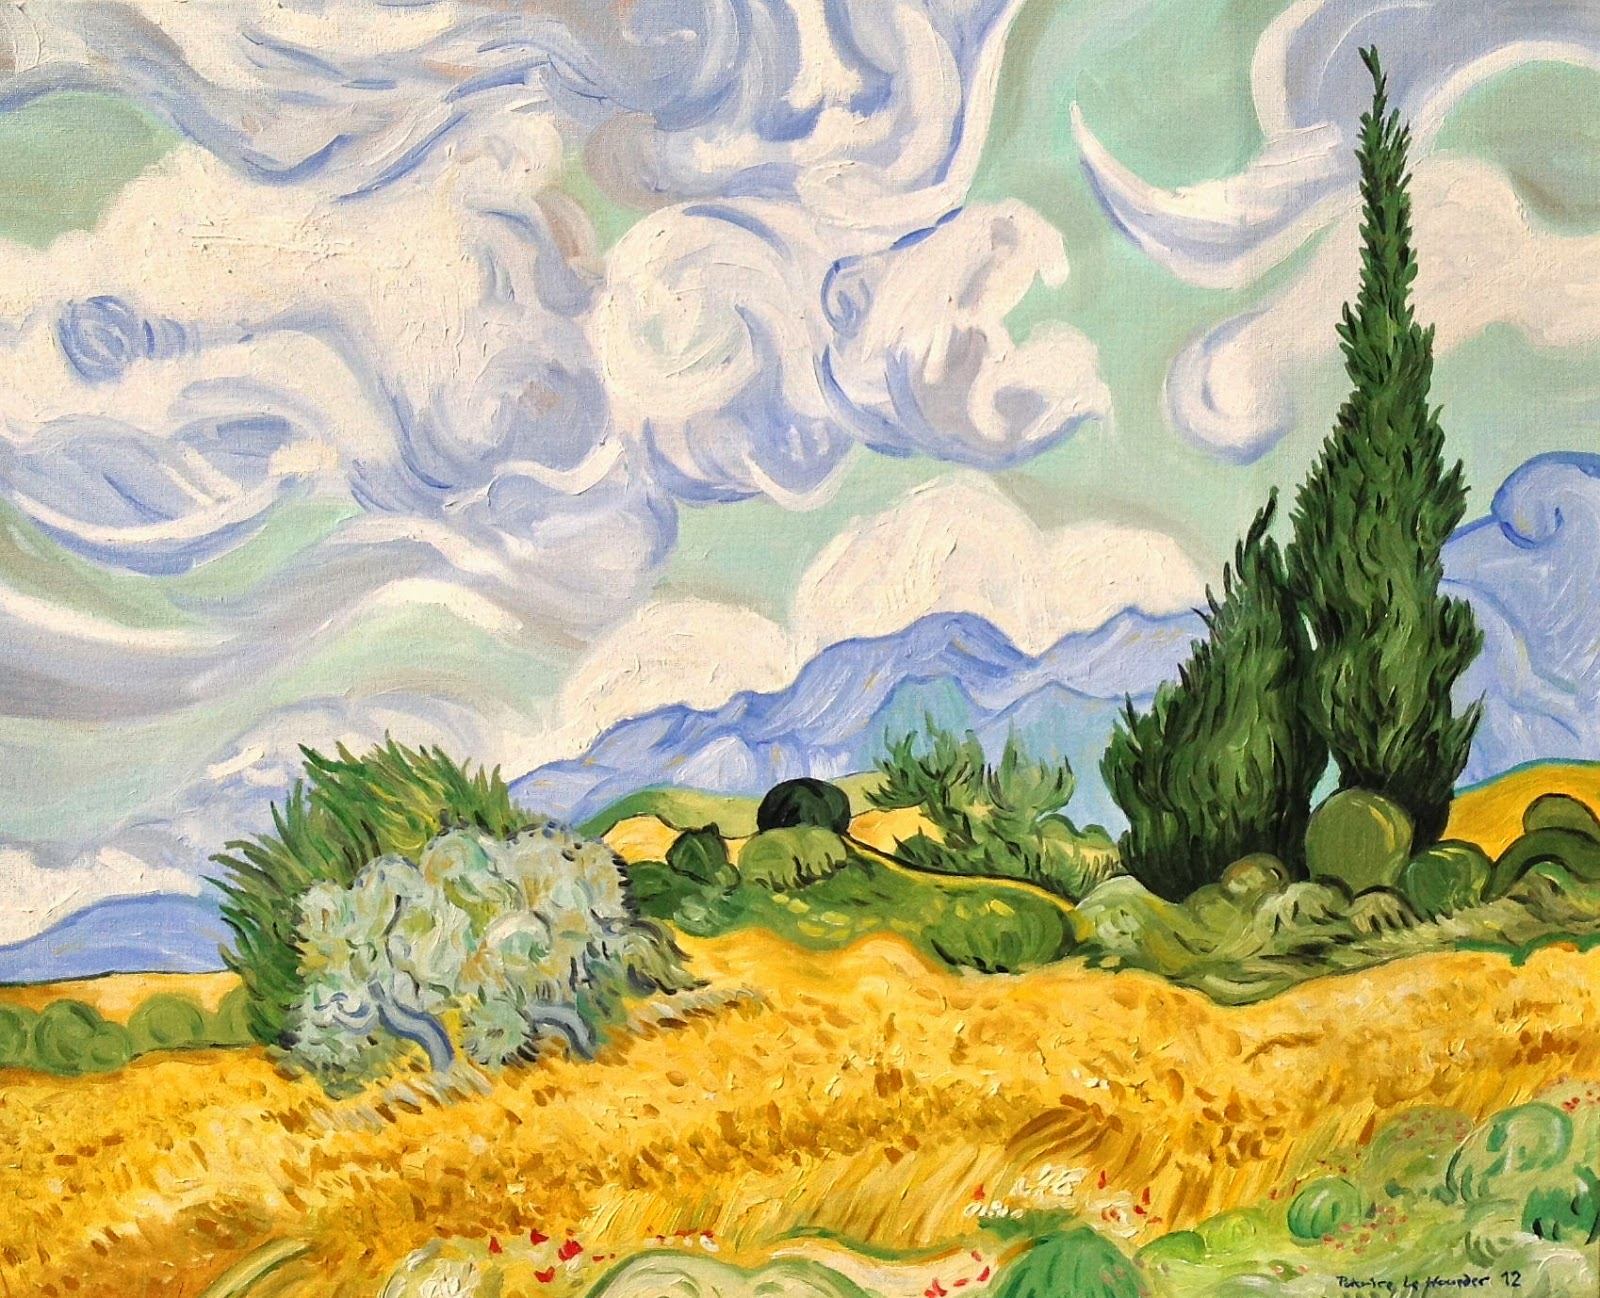
\includegraphics[scale=1.25]{v}}} % Image background
\centering
\vspace*{5cm}
\par\normalfont\fontsize{35}{35}\sffamily\selectfont
\textbf{PROGRAMMER L'INTERNET DES OBJETS }\\
{\LARGE }\par % Book title
\vspace*{1cm}
{\Huge Laurent TOUTAIN}\par % Author name
\endgroup

%----------------------------------------------------------------------------------------
%	COPYRIGHT PAGE
%----------------------------------------------------------------------------------------

\newpage
~\vfill
\thispagestyle{empty}

%\noindent Copyright \copyright\ 2014 Andrea Hidalgo\\ % Copyright notice

\noindent \textsc{IMT Atlantique}\\

\noindent Basé sur le MOOC PLIDO.\\ % License information

\noindent \textit{Publié le \today} % Printing/edition date

%----------------------------------------------------------------------------------------
%	TABLE OF CONTENTS
%----------------------------------------------------------------------------------------


\chapterimage{pano-5.jpg} % heading image

\pagestyle{empty} % No headers

\renewcommand\contentsname{Table des Matières}
\renewcommand{\bibname}{Bibliographie}

\cleardoublepage
\tableofcontents% Print the table of contents itself

%\cleardoublepage % Forces the first chapter to start on an odd page so it's on the right

\pagestyle{fancy} % Print headers again

%----------------------------------------------------------------------------------------
%	CHAPTERS
%----------------------------------------------------------------------------------------
\cleardoublepage

\chapter*{Acronymes}
\begin{multicols}{2}
\begin{acronym}
\acro{3GPP}{3rd Generation Partnership Project}
\acro{ABP}{Authentication By Personalisation}
\acro{ADSL}{Asymmetric Digital Subscriber Line}
\acro{AMQP}{Advanced Message Queuing Protocol}
\acro{AS}{Application Server}
\acro{ASCII}{American Standard Code for Information Interchange}
\acro{BLE}{Bluetooth Low Energy}
\acro{CBOR}{Concise Binaire Object Representation}
\acro{CoAP}{Constrained Application Protocol}
\acro{Cosem}{Companion Specification for Energy Management}
\acro{CRC}{Cyclic Redundancy Check}
\acro{CSV}{Comma Separated Values}
\acro{DLMS}{Device Language Message Specification}
\acro{DTT}{Digital Terrestrial Television}
\acro{DR}{Data Rate}
\acro{GSMA}{GSM Association}
\acro{HTML}{HyperText Markup Language}
\acro{HTTP}{HyperText Transport Protocol}
\acro{HTTPS}{HyperText Transport Protocol Secure}
\acro{IANA}{Internet Assigned Numbers Authority}
\acro{IBAN}{International Bank Account Number}
\acro{IEEE}{Institute of Electrical and Electronics Engineers}
\acro{IETF}{Internet Engineering Task Force}
\acro{IoT}{Internet of Things}
\acro{IP}{Internet Protocol}
\acro{IPv4}{Internet Protocol version 4}
\acro{IPv6}{Internet Protocol version 6}
\acro{IPSO}{IP for Smart Objects}
\acro{ITU}{International Telecommunication Union}
\acro{IRI}{International Resource Identifier}
\acro{ISBN}{International Standard Book Number}
\acro{ISO}{International Standardization Organization}
\acro{JMS}{Java Messaging Service}
\acro{JSON}{JavaScript Object Notation}
\acro{JSON-LD}{JavaScript Object Notation  for Linked Data}
\acro{LCIM}{Levels of Conceptual Interoperability Model}
\acro{LPWAN}{Low Power Wide Area Network}
\acro{LwM2M}{Lightweight Machine to Machine}
\acro{LNS}{LoRaWAN Network Server}
\acro{MQTT}{Message Queuing Telemetry Transport}
\acro{NAT}{Network Address Translation}
\acro{NGW}{Network GateWay}
\acro{NIDD}{Non IP Data Delivery}
\acro{OMA}{Open Mobile Alliance}
\acro{OTAA}{Over The Air Authentication}
\acro{OVH}{On Vous Herbèrge}
\acro{PAC}{Porting Authorization Code}
\acro{REST}{REpresentational State Transfer}
\acro{RFC}{Request For Comments}
\acro{RGW}{Radio GateWay}
\acro{RNIPP}{Répertoire National d'Identification des Personnes Physiques}
\acro{RSSI}{Received Signal Strength Indicator}
\acro{RTT}{Round Trip Time}
\acro{SCEF}{Service Capability Exposure Function}
\acro{SenML}{Sensor Measuring List}
\acro{SCHC}{Static Context Header Compression}
\acro{SF}{Spreading Factor}
\acro{SNR}{Signal to Noise Ratio}
\acro{SSID}{Service Set IDentifier}
\acro{STIC}{Sciences et Technologies de l’Information et de la Communication}
\acro{TCP}{Transmission Control Protocol}
\acro{TLV}{Type Length Value}
\acro{TNT}{Télévision Numérique Terrestre}
\acro{TTN}{The Things Network}
\acro{UDP}{User Datagram Protocol}
\acro{UIT}{Union internationale des télécommunications}
\acro{UNB}{Ultra Narrow-Band}
\acro{URI}{Universal Resource Identifier}
\acro{URL}{Univeral Resource Locator}
\acro{URN}{Univeral Resource Name}
\acro{VPS}{Virtual Private Server}
\acro{W3C}{World Wide Web Consortium}
\acro{WWW}{World Wide Web}
\acro{XML}{Extensible Markup Language}
\acro{XMPP}{Extensible Messaging Protocol et Presence}
\end{acronym}
\end{multicols}

%\setboolean{allchap}{true} % true: take all, false take nothing only /input

\setboolean{lfrench}{false}\setboolean{lenglish}{true}  % ENGLISH
%\setboolean{lfrench}{true}\setboolean{lenglish}{false} % FRENCH

\Input{Part00-liminaire}
\Input{Part01.0-Intro}
\Input{Part02.0-ArchiIP}
\cleardoublepage

\chapter {Wireshark}

\Index{Wireshark} va être notre ami dans la suite de cet ouvrage pour comprendre le fonctionnement des protocoles et analyser les données qui vont circuler. Malheureusement, dans certains cas, nous devons avoir recours à des outil plus rustiques comme des traces en \Index{hexadécimal}\footnote{\url{https://fr.wikipedia.org/wiki/Syst\%C3\%A8me\_hexad\%C3\%A9cimal}} (base 16).  Il faut donc se familiariser avec ces outils, ce que nous allons faire dare-dare en analysant des requêtes HTTP simples. Si vous avez accès à un ordinateur pouvant faire tourner Wireshark, nous vous recommandons d'essayer de faire les manipulation indiquées et de répondre aux questions.

\section{Installation}

L'installation de Wireshark se fait en allant sur le site éponyme \url{https://www.wireshark.org/}, soit sous Linux en installant le paquetage \texttt{wireshark}. Ce programme nécessite des droits particuliers pour accéder aux messages venant du réseau, il faut les accorder au moment de l'installation.

\section{Démarrage}

Si vous lancez Wireshark avec les bon privilèges, la fenêtre d'accueil va afficher les interfaces disponibles, comme le montre la figure~\vref{fig-wires-open} sur Windows. En regard avec le modèle de référence de l'\ac{ISO}, il s'agit des protocoles de niveau 2 présent sur l'ordinateur. Il peut s'agit d'une carte physique comme Ethernet ou Wi-Fi ou d'interface virtuelle utilisées pour communiquer en interne sur l'ordinateur. 

\begin{figure}[tbp]
\centerline{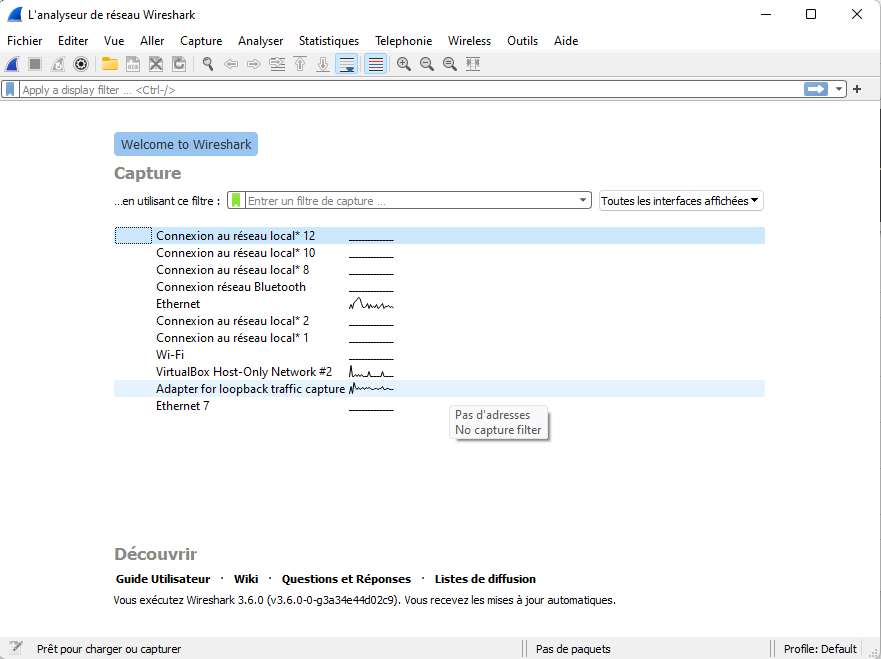
\includegraphics[width=1\columnwidth]{Pictures/wireshark-open.png}}
\caption{Ouverture de Wireshark}
\label{fig-wires-open}
\end{figure}


Il s'agit de déterminer quelle interface choisir. Ce n'est pas toujours facile car leurs noms ne sont pas toujours très explicites. Les petites courbes à gauche du nom indiquent le trafic instantané que Wireshark mesure. Sur le schéma, 3 interfaces sont actives : Ethernet, la communication avec une machine virtuelle et une interface appelée \textit{\Index{loopback}}.  La première permet d'avoir les communications avec l'extérieur et la dernière sera très utile lors des échanges entre deux processus dans cette machine.

\section {Capture}

En cliquant sur le nom de l'interface donnant accès au réseau exterieur (\index{Ethernet} dans notre cas), la fenêtre se découpe en 3 parties, comme le montre la figure~\vref{fig-wires-cap}.

\begin{figure}[tbp]
\centerline{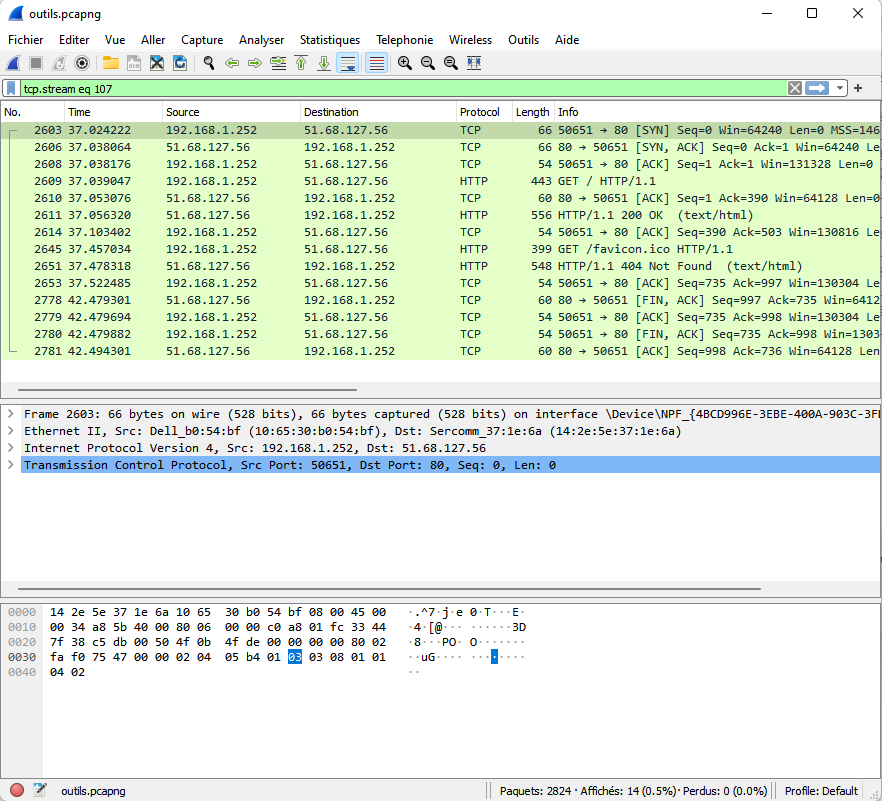
\includegraphics[width=1\columnwidth]{Pictures/ws-capture.png}}
\caption{Capture du trafic}
\label{fig-wires-cap}
\end{figure}

L'écran de Wireshark se divise en 3 parties :
\begin{itemize}
\item en haut, défile les trames qui sont capturées sur le réseau, chaque protocole à une couleur dédiée pour facilité le repérage~:
\begin{itemize}
\item le numéro de trame capturée, il s'agit d'une information ajoutée par Wireshark,
\item l'heure de capture de la trame. Cette information est aussi ajoutée par Wireshark,
\item l'adresse IP (IPv4 ou IPv6) de la machine à l'origine du paquet, 
\item l'adresse IP (IPv4 ou IPv6) de la machine destinataire du paquet,
\item le protocole de plus haut niveau contenu dans la trame. Dans notre cas, cela peut être TCP si le message TCP ne contient pas de données, comme lors de l'ouverture de connexion, ou de certains acquittements. On voit également les messages \ac{HTTP} qui sont bien entendu encapsulés dans TCP,
\item la taille en octets de la trame capturée par Wireshark,
\item finalement Wireshark fourni un résumé du contenu de la trame, pour comprendre ce qui se passe sur le réseau. Dans la capture, on retrouve pour les messages \ac{HTTP}, les requêtes GET ou les notifications ;
\end{itemize}
\item si une trame est sélectionnée dans la liste, elle apparaît dans la zone du milieu avec l'empilement protocolaire. Le contenu de chacun de ces protocoles peut être détaillé en cliquant sur le petit triangle à gauche ;
\item la fenêtre du bas donne l'équivalent en hexadécimal. Les parties surlignées correspondent aux champs sélectionnés dans la fenêtre du milieu. À noter que l'on retrouve l'information à la fois en hexadécimal et en caractère \ac{ASCII}, ce qui aide à la lecture quand on cherche une valeur spécifique.
\end{itemize}

\Question{Première colonne}
{Dans la première colonne~:
 \begin{itemize}[label=$\circ$]
   \item \Correct{Le numéro de la trame attribué par Wireshark à sa réception}
   \item \Wrong{Le numéro de la trame relevé directement dans la trame Ethernet}
  \end{itemize}
}
{
Ces numéros sont séquentiels, ils sont donc attribué localement par Wireshark. De plus il n'existe aucun champ de cette sorte dans Ethernet.
}
\Question{Deuxième colonne}
{Dans la deuxième colonne~:
 \begin{itemize}[label=$\circ$]
   \item \Correct{L'heure de réception par Wireshark}
   \item \Wrong{L'instant d'émission de la trame}
  \end{itemize}
}
{
Comme dans le cas précédent, ce numéro est ajouté par Wireshark, il n'existe pas de champ protocolaire indiquant l'instant d'émission.
}
\Question{Les troisième et quatrième colonnes}
{Dans les troisième et quatrième colonnes~:
 \begin{itemize}[label=$\circ$]
   \item \Wrong{les adresses Ethernet des machines.}
   \item \Wrong{Uniquement les adresses IPv4 des machines.}
   \item \Correct{Les adresses IPv4 ou IPv6 des machines.}
  \end{itemize}
}
{
Wireshark traite de la même manière les adresses IPv4 ou IPv6, elles sont donc affichées dans ces colonnes. L'adresse Ethernet (ou MAC) sur 48 bits n'est pas affichée par défaut dans cet écran.
}

\Question{La cinquième colonne}
{Dans la cinquième colonne~:
 \begin{itemize}[label=$\circ$]
   \item \Wrong{Le protocole applicatif (niveau 7).}
   \item \Correct{Le dernier (de plus haut niveau) protocole reconnu.}
   \item \Wrong{Le protocole de niveau 4 (ici TCP ou UDP).}
  \end{itemize}
}
{
Wireshark fournit l'information de plus haut niveau. Dans la figure~\vref{fig-wires-cap} certaines trames sont indiquées comme transportant le protocole HTTP, tandis que d'autres, généralement les acquittements sont indiqués comme étant de type TCP car elles ne transportent pas de données venant des couches supérieures.
}
\Question{La sixième colonne}
{Dans la sixième colonne~:
 \begin{itemize}[label=$\circ$]
   \item \Wrong{La taille en bits de la trame.}
   \item \Correct{La taille en octets de la trame.}
  \end{itemize}
}
{
L'unité est l'octet.
}
\Question{La septième colonne}
{Dans la septième colonne~:
 \begin{itemize}[label=$\circ$]
   \item \Correct{Un résumé des informations transportées par le protocole de plus haut niveau.}
   \item \Wrong{Les options d'IPv4.}
   \item \Wrong{le contenu en ASCII du message de plus haut niveau.}
  \end{itemize}
}
{
Wireshark cherche a interpréter les champs du protocole de plus haut niveau pour offrir un affichage synthétique de l'information.}
  \vspace{1em}

Cela fait beaucoup de trafic, nous allons limiter ce qui est affiché en ajoutant un filtre à un destinataire particulier. Le site \texttt{outils.plido.net} à l'adresse IPv4 \texttt{51.68.127.56}. Dans la fenêtre où il est indiqué \textit{Apply a display filter.} taper les instructions suivante: 

\begin{verbatim}
    ip.addr==51.68.127.56
\end{verbatim}

\noindent n'oubliez par le double \texttt{==} et la fenêtre doit devenir verte quand tout sera tapé indiquant que la syntaxe du filtre est correcte. En appuyant sur entrée, la fenêtre doit se vider.

\subsection{Analyse du trafic web}

Dans la barre d'adresse de votre navigateur préféré, taper l'URL suivante:

\begin{verbatim}
    http://outils.plido.net
\end{verbatim}

\noindent et la page Web indiqué figure~\vref{fig-firefox-hello} doit apparaître. 

\begin{figure}[tbp]
\centerline{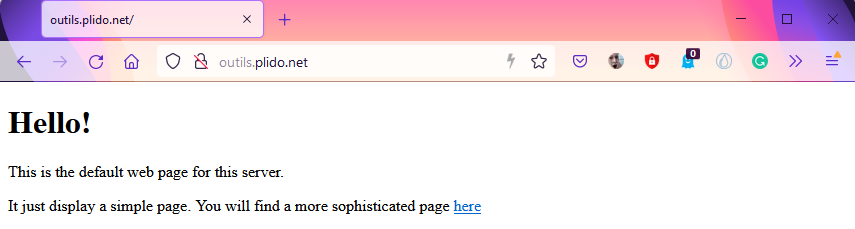
\includegraphics[width=1\columnwidth]{Pictures/firefox-simple.png}}
\caption{Afficher de la page par Firefox}
\label{fig-firefox-hello}
\end{figure}

  \vspace{1em}

Wireshark a permis de visualiser le trafic échangé entre l'ordinateur et le serveur Web. Le trafic doit être similaire a celui de la figure~\vref{fig-wires-cap}. La figure s'obtient en sélectionnant le menu \textit{Statistiques/Graphique de flux} et en cochant \textit{Limiter au Filtre d'Affichage}. Elle est un peu plus lisible car elle représente les échanges sous forme de chronographes.

\begin{figure}[tbp]
\centerline{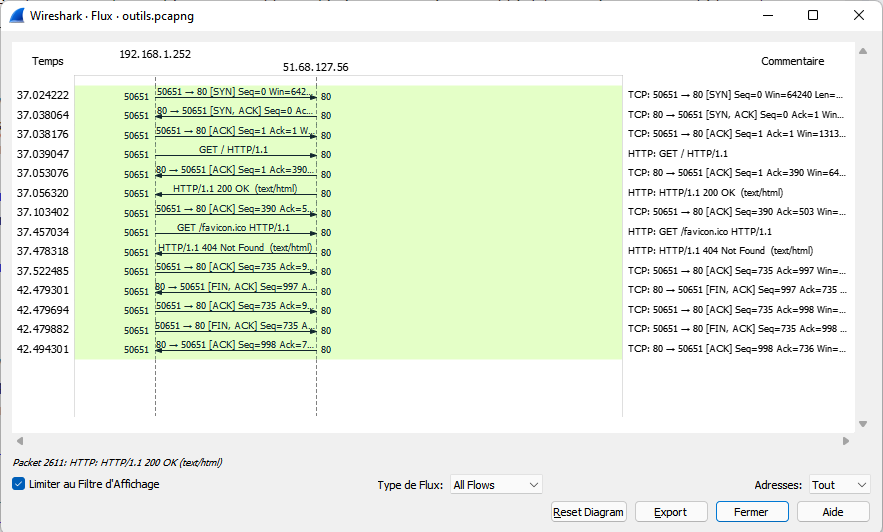
\includegraphics[width=1\columnwidth]{Pictures/ws-filtre.png}}
\caption{Diagramme temporel des échanges.}
\label{fig-ws-filtre}
\end{figure}

Trois phases peuvent être distinguées~:
\begin{itemize}
    \item L'ouverture de connexion TCP avec l'émission de trois messages TCP;
    \item la phase de transfert de données~:
    \begin{itemize}
        \item le client envoie une requête HTTP GET au serveur pour demander la ressource à la racine (\texttt{/}),
        \item le serveur acquitte le message au niveau TCP pour indiquer qu'il a bien été reçu.
        \item le serveur envoie la réponse à la requête précédente et précisant le statut (\textttt{200 : OK}) et le que contenu est formaté en HTML.
        \item le client acquitte ce message au niveau TCP
        \item le client envoie une nouvelle requête HTTP GET pour obtenir la ressource \texttt{/facicon.ico}
        \item le serveur répond que la ressource n'existe pas (\texttt{404 : Not Found}). Cette requête acquitte implicitement le message précédent.
        \item le client acquitte la réponse du serveur au niveau TCP.
    \end{itemize}
    \item le serveur termine la connexion après 5 secondes d'inactivité. La fermeture se fait en échangeant 4 messages TCP.
\end{itemize}

\Question{Code de notification de HTTP}
{Dans la trace suivante, nous avons vu que le serveur répondait aux requêtes du client par un numéro à 3 chiffres. A l'aide du \rfc{7231}, pouvez-vous attribuer le chiffre de gauche à une catégorie de notifications:
  \vspace{1em}

\tabto{3cm}
\begin{description}
    \item    0 $\square$ \tab\tab $\square$ Redirection 
    \item    1 $\square$ \tab\tab $\square$ Erreur coté serveur
    \item    2 $\square$ \tab\tab $\square$ Erreur coté client
    \item    3 $\square$ \tab\tab $\square$ Non attribué 
    \item    4 $\square$ \tab\tab $\square$ Succès
    \item    5 $\square$ \tab\tab $\square$ Information 
\end{description}

}
{
\begin{description}
    \item    0~:  Non attribué 
    \item    1~: Information 
    \item    2~: Succès
    \item    3~: Redirection
    \item    4~: Erreur coté client
    \item    5~: Erreur coté serveur
\end{description}}

\subsection{Analyse des requêtes HTTP}

La version 1.1 du protocole \ac{HTTP}  est spécifiée par le \rfc{7230}. Nous allons regarder une petite description en anglais de l'architecture et des formats des messages.

\begin{termc} [basicstyle=\footnotesize\ttfamily, frame=single]

2.  Architecture

  HTTP was created for the World Wide Web (WWW) architecture and has
  evolved over time to support the scalability needs of a worldwide
  hypertext system.  Much of that architecture is reflected in the
  terminology and syntax productions used to define HTTP.

2.1.  Client/Server Messaging

  HTTP is a stateless request/response protocol that operates by
  exchanging messages  across a reliable transport- or
  session-layer "connection".  An HTTP "client" is a
  program that establishes a connection to a server for the purpose of
  sending one or more HTTP requests.  An HTTP "server" is a program
  that accepts connections in order to service HTTP requests by sending
  HTTP responses.

\end{termc}

\Question{Organisme de standardisation.}
{
Quelle organisation de standardisation a publié ce document ?

\begin{itemize}[label=$\circ$]
   \item \Wrong{Microsoft}
   \item \Wrong{ISO}
   \item \Wrong{IEEE}
   \item \Correct{IETF}
 \end{itemize}
}
{
Le préfixe \acl{RFC} est caractéristique de l'IETF.
}
Le RFC indique ensuite :

\begin{termc} [basicstyle=\footnotesize\ttfamily, frame=singlelabel={lst-rfc7230}]
  The terms "client" and "server" refer only to the roles that these
  programs perform for a particular connection.  The same program might
  act as a client on some connections and a server on others. [...]
 
  Most HTTP communication consists of a retrieval request (GET) for a
  representation of some resource identified by a URI.  In the simplest
  case, this might be accomplished via a single bidirectional
  connection (===) between the user agent (UA) and the origin
  server (O).

           request   >
      UA ======================================= O
                                  <   response

  A client sends an HTTP request to a server in the form of a request
  message, beginning with a request-line that includes a method, URI,
  and protocol version, followed by header fields
  containing request modifiers, client information, and representation
  metadata, an empty line to indicate the end of the
  header section, and finally a message body containing the payload
  body.

  A server responds to a client's request by sending one or more HTTP
  response messages, each beginning with a status line that includes
  the protocol version, a success or error code, and textual reason
  phrase possibly followed by header fields containing
  server information, resource metadata, and representation metadata,
  an empty line to indicate the end of the header
  section, and finally a message body containing the payload body.

  The following example illustrates a typical message exchange for a
  GET request on the URI "http://www.example.com/hello.txt":

  Client request:

    GET /hello.txt HTTP/1.1
    User-Agent: curl/7.16.3 libcurl/7.16.3 OpenSSL/0.9.7l zlib/1.2.3
    Host: www.example.com
    Accept-Language: en, mi

  Server response:

    HTTP/1.1 200 OK
    Date: Mon, 27 Jul 2009 12:28:53 GMT
    Server: Apache
    Last-Modified: Wed, 22 Jul 2009 19:15:56 GMT
    ETag: "34aa387-d-1568eb00"
    Accept-Ranges: bytes
    Content-Length: 51
    Vary: Accept-Encoding
    Content-Type: text/plain

    Hello World! My payload includes a trailing CRLF.
\end{termc}

\Question{Formatage des messages HTTP}
{
Est-ce que les en-têtes HTTP ont une taille fixe (vous pouvez aller voir le \rfc{7231} qui donne des indications sur le protocole) ?
\begin{itemize}[label=$\circ$]
   \item \Wrong{l'en-tête tient en une ligne de 80 caractères.}
   \item \Correct{une ligne blanche sépare l'en-tête du contenu. L'en-tête peut contenir autant de lignes que nécessaire. }
 \end{itemize}
}
{
Comme on le voit sur l'exemple donné dans le RFC dans le message de réponse, l'en-tête HTTP contient, une ligne obligatoire, suivie d'options. Leur nombre n'est pas fixé par le standard. pour les séparer des données, une ligne blanche fait office de séparation.
}

\Question{Options des en-têtes HTTP}
{
Comment sont construites les lignes optionnelles de l'en-tête ?
\begin{itemize}[label=$\circ$]
   \item \Correct{mot-clé : valeurs}
   \item \Wrong{un texte non formaté}
   \item \Wrong{mot-clé : longueur des données : valeurs}
 \end{itemize}
}
{
L'en-tête est de taille variable. Elle comporte une première ligne obligatoire donnant la nature de la requête ou de la réponse, suivie d'informations optionnelles construites sur le format "mot clé : valeur". Une ligne blanche sépare l'en-tête du contenu.
}

\subsection{Analyse de la pile protocolaire}

La trame contenant la requête HTTP GET permet de visualiser l'encapsulation protocolaire définie par le modèle de référence de l'\ac{ISO}. Dans Wireshark, en cliquant sur la trame, on peut la voir désassemblée et en hexadécimal dans les deux fenêtres comme le montre la figure~\vref{fig-ws-GET}.

\begin{figure}[tbp]
\centerline{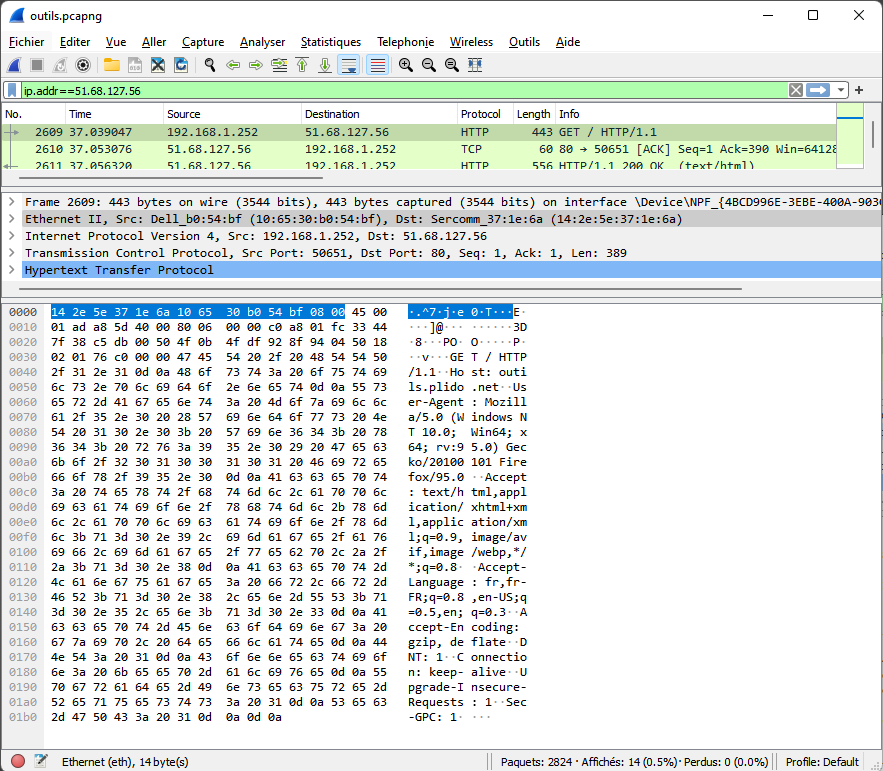
\includegraphics[width=1\columnwidth]{Pictures/ws-GET.png}}
\caption{Contenu de la trame transportant la requête HTTP GET}
\label{fig-ws-GET}
\end{figure}

  \vspace{1em}

La deuxième fenêtre montre la pile protocolaire, inversée par rapport aux représentations classique (cf. figure~\vref{fig-fullstack}), mais correspondant à l'ordre des encapsulations dans la trame. Comment Wireshark a pu arriver à un tel résultat.

\subsubsection{Ethernet}

Wireshark reçoit une trame du réseau \Index{Ethernet} ou \Index{Wi-Fi}\footnote{Pour le réseau Wi-Fi, il transforme le format en celui d'une trame Ethernet pour un affichage plus compact.}. Le format d'un trame Ethernet est défini par le standard \Index{IEEE 802.3}. L'en-tête contient trois champs~: 
\begin{itemize}
    \item 6 octets pour l'adresse MAC du destinataire,
    \item 6 octets pour l'adresse de la source.
    \item 2 octets pour le protocole de niveau supérieur. Ainsi la valeur \texttt{0x0800} désigne IPv4 et \texttt{0x86dd} IPv6.
\end{itemize}

  \vspace{1em}

Suivant le principe du modèle de référence de l'ISO, les adresses sont celles des nœuds adjacents, c'est-à-dire connecté au même réseau Ethernet ou Wi-Fi.

  \vspace{1em}

Dans notre cas, le protocole de niveau supérieur est donc un paquet IPv4 et Wireshark peut continuer à analyser, ce qui suit. Formellement se sont des données de la trame Ethernet, mais elles peuvent être comprise comme un paquet IPv4.

\Question{Mon adresse}{
Dasn l'exemple, figure~\vref{fig-ws-GET}, qu'elle est l'adresse Ethernet de la machine émettrice de la trame ?
}{
\texttt{10:65:30:b0:54:bf}. Attention, la trame commence par l'adresse de la destination, suivie de l'adresse de la source.
}

\subsubsection{IPv4}

Le format des paquets IPv4 défini dans le \rfc{791} a très peu évolué depuis sa publication en 1981. La figure~\vref{fig-header-IPv4} reprend ce format. Sans entrer dans les détails, les champs~:

\begin{itemize}
    \item adresse \texttt{source} et \texttt{destination} vont contenir les adresses IPv4 sur 32 bits des équipements d'extrémité. Des équipements intermédiaires, appelés routeur se chargent de recopier le paquet vers sa destination.
    \item Le champ \texttt{protocole} désigne la couche supérieure, la valeur 6 correspond à \Index{TCP} et 17 à \Index{UDP}.
\end{itemize}

\begin{figure}[tbp]

	\center {
    \begin{tikzpicture}

	\draw (0.5, 5.5) node  [right] {\tiny{\tt{0..................7...................15...................23....................31}}};
	
	 \draw (0.5, 5) node (context) [right, shade,  draw, minimum height=0.5cm, minimum width=1.2cm] {\tiny{Ver.}};

	\draw (1.7, 5) node (context) [right, draw, shade, minimum height=0.5cm, minimum width=1.2cm] {\tiny{IHL}};

	 \draw (2.9, 5) node (context) [right, draw, shade,  minimum height=0.5cm, minimum width=2.4cm] {\tiny{DiffServ}};

	 \draw (5.3, 5) node (context) [right, draw, shade,  minimum height=0.5cm, minimum width=4.8cm] {\tiny{Packet Length}};

	 \draw (0.5, 4.5) node (context) [right, draw, shade,  minimum height=0.5cm, minimum width=4.8cm] {\tiny{Identifier}};
	 \draw (5.3, 4.5) node (context) [right, draw, shade,  minimum height=0.5cm, minimum width=.9cm] {\tiny{flag}};
	 \draw (6.2, 4.5) node (context) [right, draw, shade,  minimum height=0.5cm, minimum width=3.9cm] {\tiny{Offset}};

	 \draw (2.9, 4) node (context) [right, draw, shade,  minimum height=0.5cm, minimum width=2.4cm, blue] {\tiny{Protocol}};

	 \draw (0.5, 4) node (context) [right, draw, shade,  minimum height=0.5cm, minimum width=2.4cm] {\tiny{TTL}};

	 \draw (5.3, 4) node (context) [right, draw, shade,  minimum height=0.5cm, minimum width=4.8cm] {\tiny{Checksum}};
	 
	 \draw (0.5, 3.5) node (context) [right, draw, shade,  minimum height=0.5cm, minimum width=9.6cm, blue] {\tiny{Source Address}};
	 \draw (0.5, 3) node (context) [right, draw, shade,  minimum height=0.5cm, minimum width=9.6cm, blue] {\tiny{Destination Address}};


	\end{tikzpicture}
	} %\center

\caption{Format d'un en-tête IPv4}
\label{fig-header-IPv4}
\end{figure}

\Question{saut par saut}{
Est-ce que l'adressse Ethernet \texttt{14:2e:5e:37:1e:6a} que l'on retrouve dans le paquet~\vref{fig-ws-GET} correspond à l'adresse Ethernet du destinataire du paquet ? A quoi correspond elle?
}{
Non, l'adresse Ethernet n'est valable que sur ce réseau Ethernet. Pour atteindre le destinataire le paquet devra traverser plusieurs routeurs. Comme la trame a été capturée sur la machine émettrice, cette adresse est donc celle du premier routeur traversé.
}

\subsubsection{TCP}

Wireshark, à partir du champ protocole valant 0x06, détermine que les données IP qui suivent l'en-tête sont un message TCP, il peut donc poursuivre le désassemblage de la trame. Le format de l'en-tête TCP est donné figure~\vref{fig-header-TCP}. Les numéros de port déterminent quelle application est utilisée. Si un client va prendre un numéro quelconque (50651 dans la trace figure~\vref{fig-ws-GET}), les serveurs vont utiliser des numéros connus de tous. Ainsi, les serveur Web se vont vus attribuer la valeur 80. Ils peuvent en choisir d'autres, comme on l'a vu lors de la constructions des \ac{URL}. 


\begin{figure}[tbp]

	\center {
    \begin{tikzpicture}

	\draw (0.5, 5.5) node  [right] {\tiny{\tt{0..................7...................15...................23....................31}}};
	
	 \draw (0.5, 5) node (SP) [right, shade,  draw, minimum height=0.5cm, minimum width=4.8cm] {};
	 \draw (SP) node [blue] {\tiny{Source Port}};

	 \draw (5.3, 5) node (DP) [right, shade,  draw, minimum height=0.5cm, minimum width=4.8cm] {};
	 \draw (DP) node [blue] {\tiny{Destination Port}};
	 
	 \draw (0.5, 4.5) node (seq) [right, shade,  draw, minimum height=0.5cm, minimum width=9.6cm] {};
	 \draw (seq) node  {\tiny{Sequence}};	 

	 \draw (0.5, 4) node (ack) [right, shade,  draw, minimum height=0.5cm, minimum width=9.6cm] {};
	 \draw (ack) node  {\tiny{Acknowledgment}};	 

	 \draw (0.5, 3.5) node (offset) [right, shade,  draw, minimum height=0.5cm, minimum width=1.2cm] {};
	 \draw (offset) node  {\tiny{Offset}};	 
	 
	 \draw (1.7, 3.5) node (res) [right, shade,  draw, minimum height=0.5cm, minimum width=1.8cm] {};
	 \draw (res) node  {\tiny{reserved}};	 
	 
	 \draw (5.3, 3.5) node (fin) [left, shade,  draw, minimum height=0.5cm, minimum width=0.3cm] {};
	 \draw (fin) node [rotate=90] {\tiny{FIN}};	 
	 \draw (5, 3.5) node (syn) [left, shade,  draw, minimum height=0.5cm, minimum width=0.3cm] {};
	 \draw (syn) node [rotate=90] {\tiny{SYN}};	 	 
	 \draw (4.7, 3.5) node (rst) [left, shade,  draw, minimum height=0.5cm, minimum width=0.3cm] {};
	 \draw (rst) node [rotate=90] {\tiny{RST}};	 	 
	 \draw (4.4, 3.5) node (psh) [left, shade,  draw, minimum height=0.5cm, minimum width=0.3cm] {};
	 \draw (psh) node [rotate=90] {\tiny{PSH}};	
	 \draw (4.1, 3.5) node (ack) [left, shade,  draw, minimum height=0.5cm, minimum width=0.3cm] {};
	 \draw (ack) node [rotate=90] {\tiny{ACK}};	
	 \draw (3.8, 3.5) node (urg) [left, shade,  draw, minimum height=0.5cm, minimum width=0.3cm] {};
	 \draw (urg) node [rotate=90] {\tiny{URG}};	
	 
	 \draw (5.3, 3.5) node (win) [right, shade,  draw, minimum height=0.5cm, minimum width=4.8cm] {};
	 \draw (win) node  {\tiny{Window}};	 	 
	 
	 \draw (0.5, 3) node (checksum) [right, shade,  draw, minimum height=0.5cm, minimum width=4.8cm] {};
	 \draw (checksum) node  {\tiny{Checksum}};

	 \draw (5.3, 3) node (urgent) [right, shade,  draw, minimum height=0.5cm, minimum width=4.8cm] {};
	 \draw (urgent) node  {\tiny{Urgent pointer}};

	 \draw (0.5, 2.5) node (option) [right,  draw, minimum height=1.5cm, minimum width=9.6cm] {};
	 \draw (option) node  {\tiny{Options}};	 	 
	 

	\end{tikzpicture}
	} %\center

\caption{Format d'un en-tête TCP}
\label{fig-header-TCP}
\end{figure}


Wireshark connaît cette liste de numéro de port bien connu et peut continuer à analyser la trame comme étant du HTTP.

Sans entrer dans les détails, on peut aussi remarquer une série de valeurs binaires qui servent par exemple à ouvrir ou fermer une connexion TCP. Si l'on reprend la phase d'ouverture de la connexion (cf. figure~\vref{fig-ws-filtre}), l'ouverture de connexion se fait par~:
\begin{itemize}
    \item l'émission par le client d'un message TCP avec le bit SYN de positionné,
    \item le serveur répond en positionnant les bits SYN et ACK dans son message,
    \item le client répond en renvoyant un message avec le bit ACK de positionné.
\end{itemize}

Ces trois messages qui ne contiennent pas de données servent à synchroniser la valeur initiale du champ \texttt{sequence} à chaque bout de la connexion.
  
\Question{Fermeture de connexion}{
A l'aide de la figure~\vref{fig-ws-GET} ou de vos captures Wireshark, quels sont les messages impliqués dans la fermeture du connexion?}
{La fermeture de déconnexion nécessite l'envoie de quatre message. L'une des extrémité, par forcement celle qui a ouvert la connexion, envoie un message avec le bit FIN positionné. Il est acquitté par l'autre entité qui a son tour envoie un message avec le bit FIN positionné qui sera acquitté pour définitivement fermer la connexion.
}   

\section{Do it yourself}\label{chap-flask}

Un serveur Web peut s'écrire en Python grâce au module \Index{Flask}. Le programme \texttt{simple\_server.py} permet de créer un serveur Web sur son ordinateur.

 \pythonlst{simple\_server.py}
 
 Ce script nécessite quelques explications :

\begin{itemize}
    \item Limport ligne 1 importe l'objet Flask à partir du module flask.
    \item A la ligne 2 une instance d'un objet Flask, c'est-à-dire un serveur web, est créée. Un nom lui est associé à des fins de débogage.
    \item A la ligne 4 contient la partie la plus délicate du script. \texttt{@} est un décorateur qui est utilisé en python pour ajouter des propriétés à une fonction. Ici, nous associons un chemin d'URI et une méthode REST à la fonction qui est ensuite définie. De cette façon, lorsque le serveur Flash recevra une requête GET sur ce chemin d'URI, il appellera la fonction \texttt{hello\_word}.
    \item La fonction texttt{hello\_word} retourne simplement un texte que le navigateur affichera.
    \item le serveur est lancé, ligne 8, en appelant la methode \pfunction{Flask}{run}. Il va attendre sur toutes les interfaces (adresse joker \texttt{0.0.0.0}) et sur le port 8080. 
\end{itemize}

  \vspace{1em}

Pour lancer le serveur, vous devez d'abord installer le module \texttt{Flask} avec \texttt{\Index{pip}}.

\begin{termc}[backgroundcolor=\color{palerod}, language=json, basicstyle=\ttfamily\small, escapechar=@]
# @\textbf{pip3 install Flask}@
Collecting Flask
  Downloading Flask-2.0.2-py3-none-any.whl (95 kB)
     |                                  | 95 kB 4.3 MB/s 
Collecting Jinja2>=3.0
  Downloading Jinja2-3.0.3-py3-none-any.whl (133 kB)
...
\end{termc}

  \vspace{1em}

Une fois le paquetage installé, il suffit d'exécuter le programme:
\begin{termc}[backgroundcolor=\color{palerod}, language=json, basicstyle=\ttfamily\small, escapechar=@]
# @\textbf{python3.9 simple\_server.py}@
 * Serving Flask app 'My First Web Server' (lazy loading)
 * Environment: production
   WARNING: This is a development server. Do not use it in a production
   deployment.
   Use a production WSGI server instead.
 * Debug mode: off
 * Running on all addresses.
   WARNING: This is a development server. Do not use it in a production
   deployment.
 * Running on http://192.168.1.53:8080/ (Press CTRL+C to quit)
127.0.0.1 - - [14/Dec/2021 21:06:55] "GET / HTTP/1.1" 200 -
127.0.0.1 - - [14/Dec/2021 21:06:59] "GET /favicon.ico HTTP/1.1" 404 -
\end{termc}


\Question{loopback}
{Quelle URI devez vous entrer dans votre navigateur pour accéder en local à ce serveur.}
{L'adresse de loopback est \texttt{127.0.0.1} et le port est 8080, le chemin d'URI est \texttt{/}. L'URI est donc \texttt{http://127.0.0.1:8080/}.}

\Question{Nom du serveur}{
A l'aide de Wireshark, pouvez vous déterminer dans la réponse les valeurs des options HTTP \texttt{\Index{Content-Type}} et \texttt{Server}.

Ne pas oublier que le trafic passe par l'interface \textit{loopback}. Pour afficher le trafic sur un port particulier, vous pouvez utiliser le filtre \texttt{tcp.port==XXXX}.
}{
On trouve les valeurs suivantes~:
\begin{itemize}
    \item \texttt{Server: Werkzeug/2.0.2 Python/3.9.6}
    \item \texttt{Content-Type: text/html; charset=utf-8}. La ressource est codée en HTML en utilisant un codage ASCII sur 8 bits.
\end{itemize}
}
\Input{Part03.0-Modbus}
\Input{Part04.0-ArchiIoT}
\Input{Part05.0-Data}
\Input{Part06.0-VSensors}
\Input{Part06.5-beebotte}
\Input{Part07.0-LoPy}
\Input{Part08.0-Sigfox}
\Input{Part09.0-LoRaWAN}
\Input{Part10.0-CoAP}
\Input{Part10.5-aiocoap}
\Input{Part11.0-LwM2M}






%%%%%%%%%%%%%%%%%%%%%%%%%%%%%%%%%%%%%



\immediate\closeout\tempfile
\setboolean{Response}{false}

\cleardoublepage
\chapter{Réponses aux questions}
\input{questions}

\cleardoublepage
\printindex

\cleardoublepage
\printbibliography

\end{document}